\section{Conclusión}
Al analizar los resultados del proyecto, se observa el logro de este mismo al 
cumplir con los objetivos planeados donde el sistema es capaz de realizar un 
conjunto de mediciones y calculos para advertir al usuario de un posible riesgo al infante.
Ademas este proyecto observa el problema de la asfixia desde el punto de vista de un 
dispositivo adherido al infante proporcionando una visión distinta a sus contrapartes 
mencionadas en nuestra investigación inicial.
Como ultimo se observaron ciertas restricciones y limitaciones debido aspectos 
de la situación global en donde hay una crisis de chips de silicio, lo que genero 
una limitante en la seleccion de los sensores principales, lo que a su vez genero 
una restriccion en la capacidad del dispositivo para detectar los movimientos.
Con base a estas conclusiones, futuros desarrollos pueden proporcionar una mayor 
miniaturización ademas de una capacidad de los sensores mayores, mejorando su 
funcionamiento y disminuyendo las dificultades que representa la medición de la
posición del infante utilizando sensores giroscopicos, acelerometros y magnetometros

\begin{figure}[htp!]
    \centering
    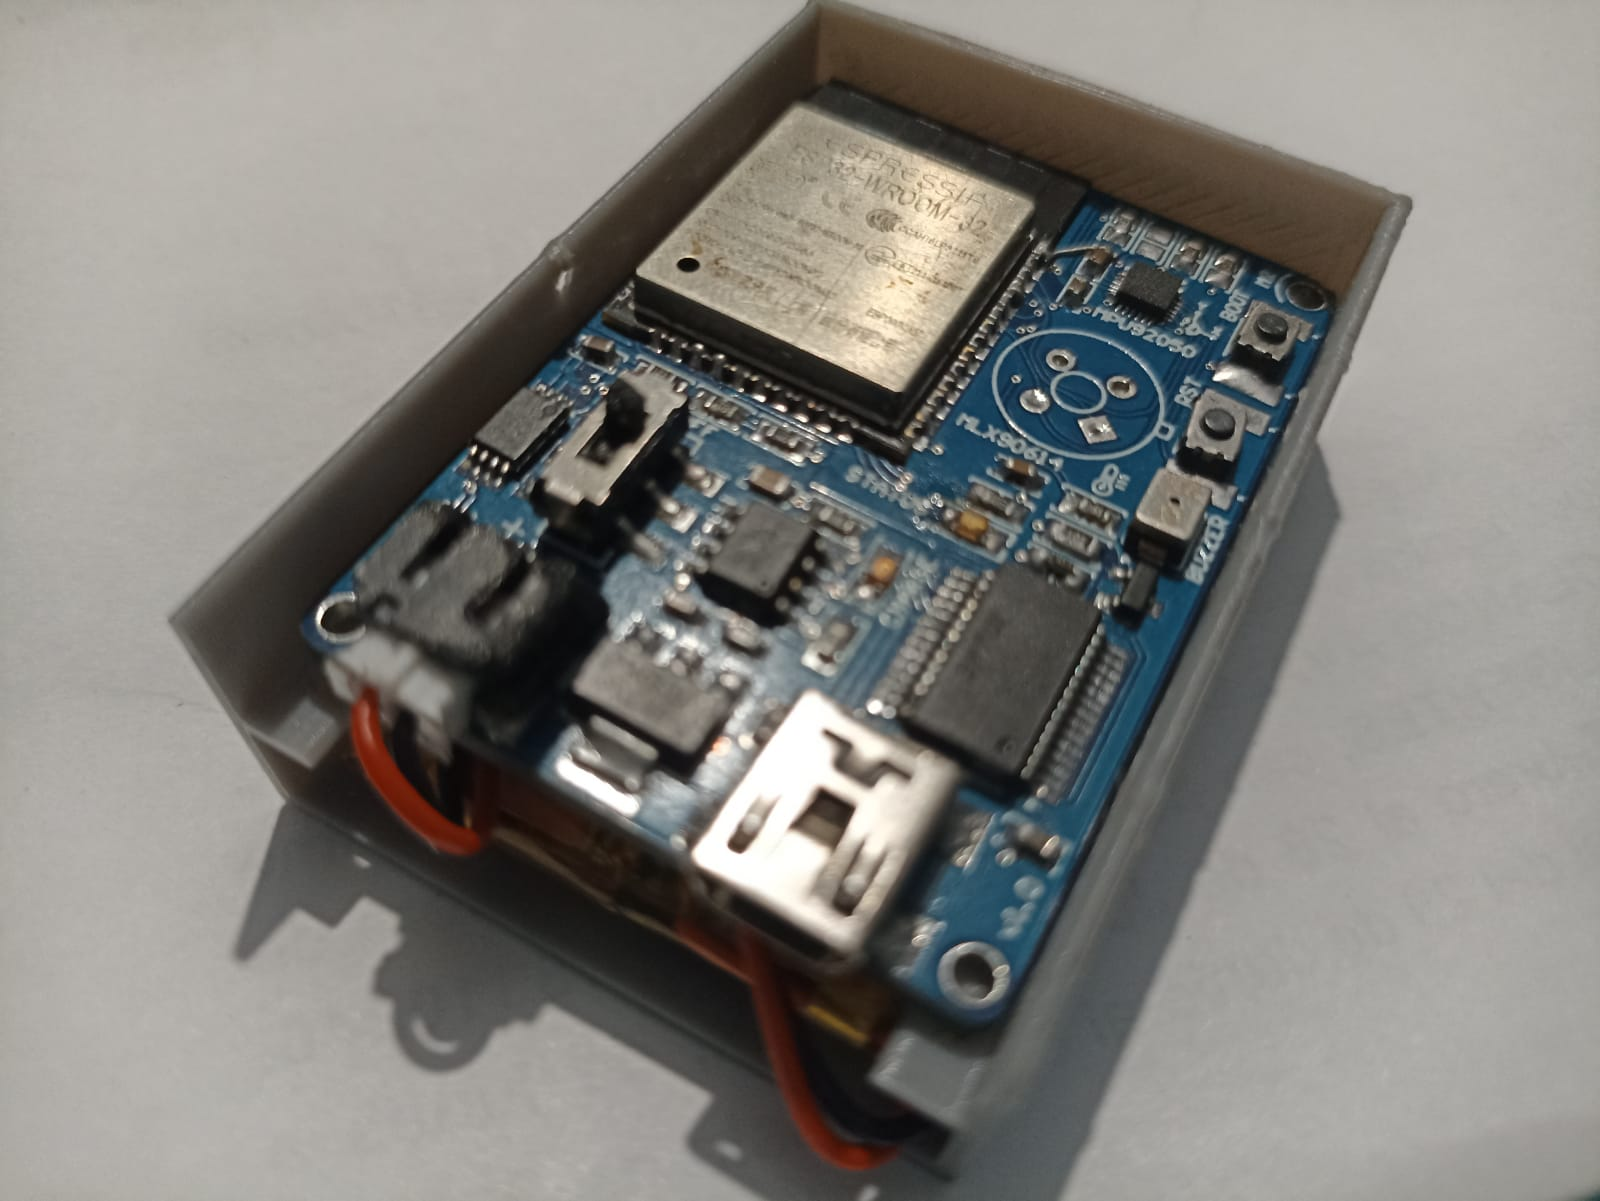
\includegraphics[width=\columnwidth]{final_device.jpg}
    \caption{Dispositivo final}
    \label{fig: final_device}
\end{figure}
\FloatBarrier